\documentclass[12pt,a4paper]{article}
\usepackage[utf8]{inputenc}
\usepackage[english]{babel}
\usepackage{geometry}
\usepackage{fancyhdr}
\usepackage{graphicx}
\usepackage{float}
\usepackage{tabularx}
\usepackage{longtable}
\usepackage{array}
\usepackage{booktabs}
\usepackage{multirow}
\usepackage{listings}
\usepackage{xcolor}
\usepackage{tikz}
\usepackage{forest}
\usepackage{hyperref}
\usepackage{amsmath}
\usepackage{amsfonts}
\usepackage{amssymb}
\usepackage{enumitem}
\usepackage{caption}
\usepackage{subcaption}

% Page setup
\geometry{
    left=2.5cm,
    right=2.5cm,
    top=2.5cm,
    bottom=2.5cm
}

% Header and footer
\pagestyle{fancy}
\fancyhf{}
\rhead{HIV Clinic Management System}
\lhead{Software Design Specification}
\cfoot{\thepage}

% Code listing style
\lstset{
    basicstyle=\ttfamily\small,
    breaklines=true,
    frame=single,
    language=Java,
    numbers=left,
    numberstyle=\tiny,
    showstringspaces=false,
    tabsize=2,
    commentstyle=\color{gray},
    keywordstyle=\color{blue},
    stringstyle=\color{red}
}

% TikZ libraries
\usetikzlibrary{shapes.geometric, arrows, positioning, fit, backgrounds}

% Define colors
\definecolor{packagecolor}{RGB}{173, 216, 230}
\definecolor{classcolor}{RGB}{255, 218, 185}
\definecolor{interfacecolor}{RGB}{221, 160, 221}

% Title page
\title{
    \vspace{-2cm}
    \Huge\textbf{HIV Clinic Management System}\\
    \vspace{1cm}
    \Large\textbf{Software Design Specification}\\
    \vspace{2cm}
    \normalsize Version 1.0
}

\author{}
\date{
    \vspace{4cm}
    – Ho Chi Minh City, January 2025 –
}

\begin{document}

\maketitle
\thispagestyle{empty}

\newpage

% Record of changes
\section*{Record of Changes}
\begin{longtable}{|p{3cm}|p{2cm}|p{3cm}|p{6cm}|}
\hline
\textbf{Date} & \textbf{A*M, D} & \textbf{In charge} & \textbf{Change Description} \\
\hline
2025-01-07 & A & System Architect & Initial creation of SDS document \\
\hline
2025-01-07 & A & System Architect & Added comprehensive system architecture \\
\hline
2025-01-07 & A & System Architect & Added detailed class diagrams and specifications \\
\hline
2025-01-07 & A & System Architect & Added database design and API documentation \\
\hline
\end{longtable}

\footnotesize{*A - Added, M - Modified, D - Deleted}

\newpage

% Table of contents
\tableofcontents

\newpage

\section{Overview}

\subsection{Code Packages}

The HIV Clinic Management System follows a layered architecture pattern with clear separation of concerns. The backend is built using Spring Boot framework with Java 17, while the frontend uses React with modern JavaScript (ES6+). The system implements a comprehensive package structure that promotes maintainability and scalability.

\begin{figure}[H]
\centering
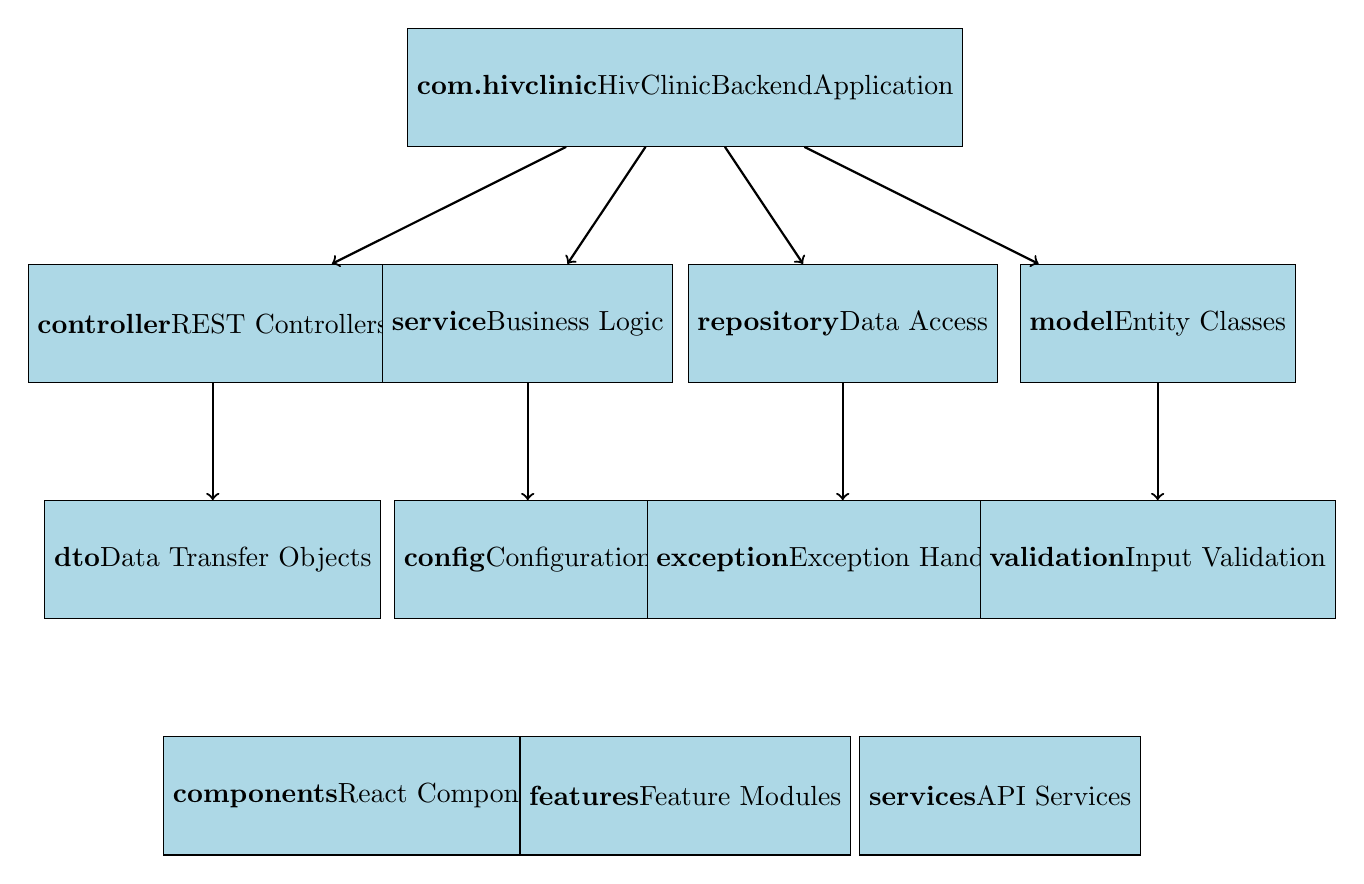
\begin{tikzpicture}[
    package/.style={draw, fill=packagecolor, minimum width=3cm, minimum height=1.5cm, text centered},
    arrow/.style={->, thick}
]

% Main application package
\node[package] (main) at (0, 0) {\textbf{com.hivclinic}\\HivClinicBackendApplication};

% Layer packages
\node[package] (controller) at (-6, -3) {\textbf{controller}\\REST Controllers};
\node[package] (service) at (-2, -3) {\textbf{service}\\Business Logic};
\node[package] (repository) at (2, -3) {\textbf{repository}\\Data Access};
\node[package] (model) at (6, -3) {\textbf{model}\\Entity Classes};

% Supporting packages
\node[package] (dto) at (-6, -6) {\textbf{dto}\\Data Transfer Objects};
\node[package] (config) at (-2, -6) {\textbf{config}\\Configuration};
\node[package] (exception) at (2, -6) {\textbf{exception}\\Exception Handling};
\node[package] (validation) at (6, -6) {\textbf{validation}\\Input Validation};

% Frontend packages
\node[package] (components) at (-4, -9) {\textbf{components}\\React Components};
\node[package] (features) at (0, -9) {\textbf{features}\\Feature Modules};
\node[package] (services) at (4, -9) {\textbf{services}\\API Services};

% Arrows
\draw[arrow] (main) -- (controller);
\draw[arrow] (main) -- (service);
\draw[arrow] (main) -- (repository);
\draw[arrow] (main) -- (model);

\draw[arrow] (controller) -- (dto);
\draw[arrow] (service) -- (config);
\draw[arrow] (repository) -- (exception);
\draw[arrow] (model) -- (validation);

\end{tikzpicture}
\caption{Package Structure Overview}
\label{fig:package-structure}
\end{figure}

\begin{table}[H]
\centering
\caption{Package Descriptions}
\label{tab:package-descriptions}
\begin{tabularx}{\textwidth}{|c|l|X|}
\hline
\textbf{No} & \textbf{Package} & \textbf{Description} \\
\hline
01 & com.hivclinic.controller & REST API endpoints handling HTTP requests and responses. Contains controllers for authentication, appointments, user management, and ARV treatments. \\
\hline
02 & com.hivclinic.service & Business logic layer implementing core application functionality. Handles appointment scheduling, notification management, and user authentication. \\
\hline
03 & com.hivclinic.repository & Data access layer using Spring Data JPA. Provides database operations for all entity classes with custom queries for complex operations. \\
\hline
04 & com.hivclinic.model & JPA entity classes representing database tables. Includes User, Appointment, ARVTreatment, Notification, and related entities. \\
\hline
05 & com.hivclinic.dto & Data Transfer Objects for API communication. Separate request and response DTOs for clean API contracts. \\
\hline
06 & com.hivclinic.config & Spring configuration classes including security, JWT, CORS, and database configuration. \\
\hline
07 & com.hivclinic.exception & Custom exception classes and global exception handling for consistent error responses. \\
\hline
08 & com.hivclinic.validation & Custom validation annotations and validators for input validation. \\
\hline
09 & com.hivclinic.mapper & Object mapping utilities for converting between entities and DTOs. \\
\hline
10 & components & React components organized by functionality: layout, notifications, scheduling, and ARV treatment management. \\
\hline
11 & features & Feature-based React modules for Admin, Doctor, Patient, and Manager dashboards. \\
\hline
12 & services & Frontend API service layer for HTTP communication with the backend REST API. \\
\hline
\end{tabularx}
\end{table}

\subsection{Database Design}

\subsubsection{Database Schema}

The HIV Clinic Management System uses Microsoft SQL Server as the primary database. The schema follows 3rd Normal Form (3NF) design principles with proper referential integrity constraints.

\begin{figure}[H]
\centering
\fbox{
\begin{minipage}{0.9\textwidth}
\centering
\vspace{3cm}
\textbf{HIV Clinic Management System - Database Schema ERD}\\
\vspace{0.5cm}
\textit{Comprehensive Entity-Relationship Diagram showing all database tables, their relationships, primary keys, foreign keys, and cardinality constraints for the HIV clinic management system}\\
\vspace{0.5cm}
\textit{Dimensions: 24" x 18"}\\
\vspace{0.5cm}
\textit{Generated from: database\_schema\_erd.mermaid}\\
\vspace{3cm}
\end{minipage}
}
\caption{Database Entity-Relationship Diagram}
\label{fig:database-erd}
\end{figure}

\subsubsection{Core Entity Classes}

\begin{longtable}{|p{2cm}|p{3cm}|p{9cm}|}
\hline
\textbf{Entity} & \textbf{Table Name} & \textbf{Description} \\
\hline
User & Users & Central user entity with authentication and role management \\
\hline
Role & Roles & System role definitions for access control \\
\hline
PatientProfile & PatientProfiles & Extended patient information and demographics \\
\hline
DoctorProfile & DoctorProfiles & Doctor professional information and specialties \\
\hline
Appointment & Appointments & Appointment scheduling and management \\
\hline
DoctorAvailabilitySlot & DoctorAvailabilitySlots & Doctor availability time slot management \\
\hline
PatientRecord & PatientRecords & Comprehensive medical records \\
\hline
ARVTreatment & ARVTreatments & HIV antiretroviral treatment tracking \\
\hline
MedicationRoutine & MedicationRoutines & Daily medication schedules \\
\hline
Notification & Notifications & System notification management \\
\hline
NotificationTemplate & NotificationTemplates & Reusable notification templates \\
\hline
UserSession & UserSessions & User session management \\
\hline
LoginActivity & LoginActivity & Login activity tracking \\
\hline
SystemSetting & SystemSettings & System configuration settings \\
\hline
\end{longtable}

\section{System Architecture}

\subsection{High-Level Architecture}

The HIV Clinic Management System implements a modern three-tier architecture with clear separation between presentation, business logic, and data layers.

\begin{figure}[H]
\centering
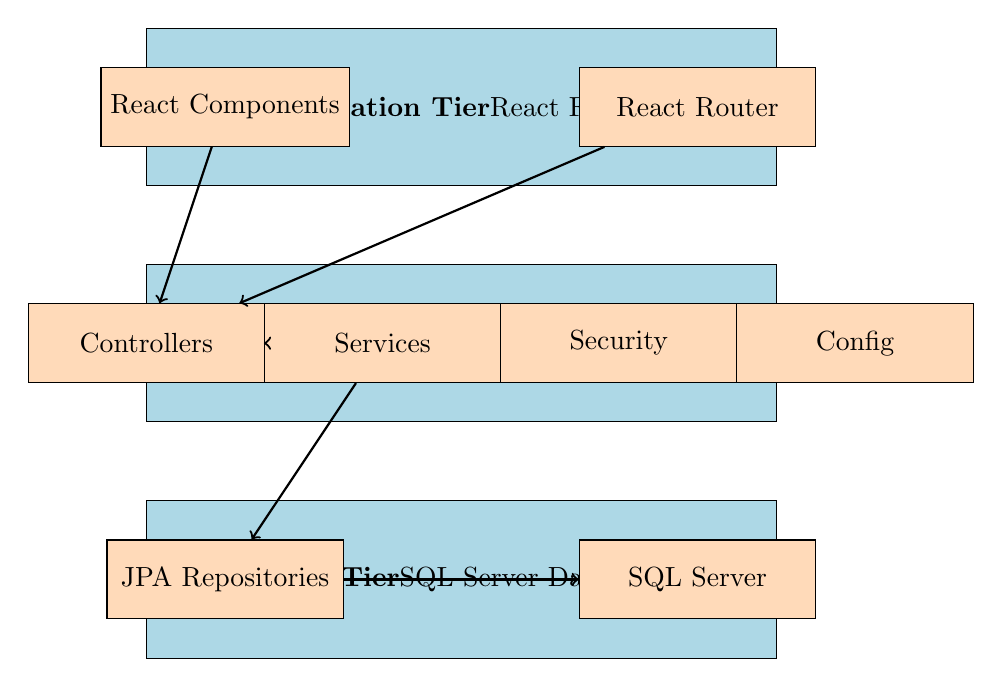
\begin{tikzpicture}[
    tier/.style={draw, fill=packagecolor, minimum width=8cm, minimum height=2cm, text centered},
    component/.style={draw, fill=classcolor, minimum width=3cm, minimum height=1cm, text centered},
    arrow/.style={->, thick}
]

% Tiers
\node[tier] (presentation) at (0, 4) {\textbf{Presentation Tier}\\React Frontend};
\node[tier] (business) at (0, 1) {\textbf{Business Logic Tier}\\Spring Boot Backend};
\node[tier] (data) at (0, -2) {\textbf{Data Tier}\\SQL Server Database};

% Components
\node[component] (react) at (-3, 4) {React Components};
\node[component] (router) at (3, 4) {React Router};

\node[component] (controller) at (-4, 1) {Controllers};
\node[component] (service) at (-1, 1) {Services};
\node[component] (security) at (2, 1) {Security};
\node[component] (config) at (5, 1) {Config};

\node[component] (jpa) at (-3, -2) {JPA Repositories};
\node[component] (sql) at (3, -2) {SQL Server};

% Arrows
\draw[arrow] (react) -- (controller);
\draw[arrow] (router) -- (controller);
\draw[arrow] (controller) -- (service);
\draw[arrow] (service) -- (jpa);
\draw[arrow] (jpa) -- (sql);

\end{tikzpicture}
\caption{System Architecture Overview}
\label{fig:system-architecture}
\end{figure}

\subsection{Component Architecture}

\begin{figure}[H]
\centering
\fbox{
\begin{minipage}{0.9\textwidth}
\centering
\vspace{3cm}
\textbf{HIV Clinic Management System - Component Diagram}\\
\vspace{0.5cm}
\textit{Comprehensive component diagram showing all system components, their interfaces, dependencies, and communication patterns between frontend React components, backend Spring Boot services, and database layer}\\
\vspace{0.5cm}
\textit{Dimensions: 20" x 16"}\\
\vspace{0.5cm}
\textit{Generated from: component\_diagram.plantuml}\\
\vspace{3cm}
\end{minipage}
}
\caption{System Component Diagram}
\label{fig:component-diagram}
\end{figure}

\section{Detailed Design}

\subsection{Authentication System}

\subsubsection{JWT Token Management}

The system implements JWT-based authentication with secure token generation, validation, and refresh mechanisms.

\begin{lstlisting}[language=Java, caption=JWT Token Configuration]
@Configuration
@EnableWebSecurity
public class SecurityConfig {
    
    @Autowired
    private JwtAuthenticationEntryPoint jwtAuthenticationEntryPoint;
    
    @Autowired
    private UserDetailsService jwtUserDetailsService;
    
    @Autowired
    private JwtRequestFilter jwtRequestFilter;
    
    @Bean
    public PasswordEncoder passwordEncoder() {
        return new BCryptPasswordEncoder();
    }
    
    @Bean
    public AuthenticationManager authenticationManager(
            AuthenticationConfiguration authConfig) throws Exception {
        return authConfig.getAuthenticationManager();
    }
}
\end{lstlisting}

\subsubsection{User Authentication Flow}

\begin{figure}[H]
\centering
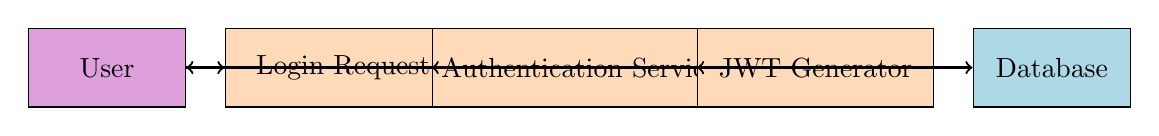
\begin{tikzpicture}[
    actor/.style={draw, fill=interfacecolor, minimum width=2cm, minimum height=1cm},
    process/.style={draw, fill=classcolor, minimum width=3cm, minimum height=1cm},
    data/.style={draw, fill=packagecolor, minimum width=2cm, minimum height=1cm},
    arrow/.style={->, thick}
]

% Actors and processes
\node[actor] (user) at (-6, 0) {User};
\node[process] (login) at (-3, 0) {Login Request};
\node[process] (auth) at (0, 0) {Authentication Service};
\node[process] (jwt) at (3, 0) {JWT Generator};
\node[data] (db) at (6, 0) {Database};

% Flow
\draw[arrow] (user) -- (login);
\draw[arrow] (login) -- (auth);
\draw[arrow] (auth) -- (db);
\draw[arrow] (auth) -- (jwt);
\draw[arrow] (jwt) -- (user);

\end{tikzpicture}
\caption{Authentication Flow}
\label{fig:auth-flow}
\end{figure}

\subsection{Appointment Management System}

\subsubsection{Appointment Booking Process}

The appointment booking system handles the complete lifecycle of appointment scheduling, including availability checking, conflict resolution, and notification management.

\begin{figure}[H]
\centering
\fbox{
\begin{minipage}{0.9\textwidth}
\centering
\vspace{3cm}
\textbf{HIV Clinic Management System - Appointment Booking Sequence}\\
\vspace{0.5cm}
\textit{Detailed sequence diagram showing the appointment booking process from patient request through doctor availability checking, appointment creation, notification scheduling, and confirmation}\\
\vspace{0.5cm}
\textit{Dimensions: 22" x 14"}\\
\vspace{0.5cm}
\textit{Generated from: appointment\_booking\_sequence.mermaid}\\
\vspace{3cm}
\end{minipage}
}
\caption{Appointment Booking Sequence Diagram}
\label{fig:appointment-sequence}
\end{figure}

\subsubsection{Appointment Entity Design}

\begin{lstlisting}[language=Java, caption=Appointment Entity]
@Entity
@Table(name = "Appointments")
@Data
@NoArgsConstructor
@AllArgsConstructor
public class Appointment {
    
    @Id
    @GeneratedValue(strategy = GenerationType.IDENTITY)
    @Column(name = "AppointmentID")
    private Integer appointmentId;
    
    @ManyToOne(fetch = FetchType.LAZY)
    @JoinColumn(name = "PatientUserID", nullable = false)
    @JsonIgnoreProperties({"hibernateLazyInitializer", "handler", "passwordHash"})
    private User patientUser;
    
    @ManyToOne(fetch = FetchType.LAZY)
    @JoinColumn(name = "DoctorUserID", nullable = false)
    @JsonIgnoreProperties({"hibernateLazyInitializer", "handler", "passwordHash"})
    private User doctorUser;
    
    @Column(name = "AppointmentDateTime", nullable = false)
    @JsonFormat(pattern = "yyyy-MM-dd'T'HH:mm:ss")
    private LocalDateTime appointmentDateTime;
    
    @Column(name = "Status", nullable = false, length = 50)
    private String status = "Scheduled";
    
    @Column(name = "DurationMinutes")
    private Integer durationMinutes = 30;
}
\end{lstlisting}

\subsection{ARV Treatment Management}

\subsubsection{Treatment Tracking System}

The ARV treatment management system provides comprehensive tracking of HIV antiretroviral treatments, including medication schedules, adherence monitoring, and side effect tracking.

\begin{figure}[H]
\centering
\fbox{
\begin{minipage}{0.9\textwidth}
\centering
\vspace{3cm}
\textbf{HIV Clinic Management System - ARV Treatment Class Diagram}\\
\vspace{0.5cm}
\textit{Comprehensive class diagram showing ARV treatment entities, their relationships, attributes, and methods for managing HIV treatment regimens, medication routines, and patient adherence tracking}\\
\vspace{0.5cm}
\textit{Dimensions: 24" x 18"}\\
\vspace{0.5cm}
\textit{Generated from: arv\_treatment\_class\_diagram.plantuml}\\
\vspace{3cm}
\end{minipage}
}
\caption{ARV Treatment Class Diagram}
\label{fig:arv-treatment-class}
\end{figure}

\subsubsection{ARV Treatment Entity}

\begin{lstlisting}[language=Java, caption=ARV Treatment Entity]
@Entity
@Table(name = "ARVTreatments")
@Data
@NoArgsConstructor
@AllArgsConstructor
public class ARVTreatment {
    
    @Id
    @GeneratedValue(strategy = GenerationType.IDENTITY)
    @Column(name = "ARVTreatmentID")
    private Integer arvTreatmentId;
    
    @ManyToOne(fetch = FetchType.LAZY)
    @JoinColumn(name = "PatientUserID", nullable = false)
    @JsonIgnoreProperties({"hibernateLazyInitializer", "handler"})
    private User patientUser;
    
    @ManyToOne(fetch = FetchType.LAZY)
    @JoinColumn(name = "DoctorUserID", nullable = false)
    @JsonIgnoreProperties({"hibernateLazyInitializer", "handler"})
    private User doctorUser;
    
    @Column(name = "MedicationName", nullable = false)
    private String medicationName;
    
    @Column(name = "Dosage", nullable = false)
    private String dosage;
    
    @Column(name = "Frequency", nullable = false)
    private String frequency;
    
    @Column(name = "StartDate", nullable = false)
    @JsonFormat(pattern = "yyyy-MM-dd")
    private LocalDate startDate;
    
    @Column(name = "EndDate")
    @JsonFormat(pattern = "yyyy-MM-dd")
    private LocalDate endDate;
    
    @Column(name = "IsActive", nullable = false)
    private Boolean isActive = true;
    
    @Column(name = "SideEffects", columnDefinition = "NVARCHAR(MAX)")
    private String sideEffects;
    
    @Column(name = "DoctorNotes", columnDefinition = "NVARCHAR(MAX)")
    private String doctorNotes;
}
\end{lstlisting}

\subsection{Notification System}

\subsubsection{Notification Architecture}

The notification system provides automated reminders for appointments and medication adherence, with configurable templates and delivery mechanisms.

\begin{figure}[H]
\centering
\fbox{
\begin{minipage}{0.9\textwidth}
\centering
\vspace{3cm}
\textbf{HIV Clinic Management System - Notification System Class Diagram}\\
\vspace{0.5cm}
\textit{Comprehensive class diagram showing notification entities, template management, scheduling system, and delivery mechanisms for appointment reminders and medication alerts}\\
\vspace{0.5cm}
\textit{Dimensions: 22" x 16"}\\
\vspace{0.5cm}
\textit{Generated from: notification\_class\_diagram.plantuml}\\
\vspace{3cm}
\end{minipage}
}
\caption{Notification System Class Diagram}
\label{fig:notification-class}
\end{figure}

\subsubsection{Notification Entity}

\begin{lstlisting}[language=Java, caption=Notification Entity]
@Entity
@Table(name = "Notifications")
@Data
@NoArgsConstructor
@AllArgsConstructor
public class Notification {
    
    @Id
    @GeneratedValue(strategy = GenerationType.IDENTITY)
    @Column(name = "NotificationID")
    private Integer notificationId;
    
    @ManyToOne(fetch = FetchType.LAZY)
    @JoinColumn(name = "UserID", nullable = false)
    @JsonIgnoreProperties({"hibernateLazyInitializer", "handler"})
    private User user;
    
    @Column(name = "Title", nullable = false)
    private String title;
    
    @Column(name = "Message", nullable = false, columnDefinition = "NVARCHAR(MAX)")
    private String message;
    
    @Column(name = "Type", nullable = false)
    private String type; // APPOINTMENT, MEDICATION, SYSTEM
    
    @Column(name = "IsRead", nullable = false)
    private Boolean isRead = false;
    
    @Column(name = "CreatedAt", nullable = false)
    @JsonFormat(pattern = "yyyy-MM-dd'T'HH:mm:ss")
    private LocalDateTime createdAt;
    
    @Column(name = "ScheduledFor")
    @JsonFormat(pattern = "yyyy-MM-dd'T'HH:mm:ss")
    private LocalDateTime scheduledFor;
    
    @ManyToOne(fetch = FetchType.LAZY)
    @JoinColumn(name = "templateId")
    @JsonIgnoreProperties({"hibernateLazyInitializer", "handler"})
    private NotificationTemplate template;
}
\end{lstlisting}

\section{API Design}

\subsection{REST API Endpoints}

The system provides comprehensive REST API endpoints organized by functionality:

\begin{longtable}{|p{3cm}|p{2cm}|p{3cm}|p{8cm}|}
\hline
\textbf{Endpoint} & \textbf{Method} & \textbf{Path} & \textbf{Description} \\
\hline
Authentication & POST & /api/auth/login & User login with JWT token generation \\
\hline
Authentication & POST & /api/auth/register & User registration with role assignment \\
\hline
Authentication & GET & /api/auth/me & Get current user profile \\
\hline
Authentication & PUT & /api/auth/profile & Update user profile information \\
\hline
Appointments & POST & /api/appointments/book & Book new appointment \\
\hline
Appointments & GET & /api/appointments/patient/my-appointments & Get patient's appointments \\
\hline
Appointments & GET & /api/appointments/doctor/my-appointments & Get doctor's appointments \\
\hline
Appointments & PUT & /api/appointments/{id}/cancel & Cancel appointment \\
\hline
ARV Treatments & GET & /api/arv-treatments/my-treatments & Get patient's treatments \\
\hline
ARV Treatments & POST & /api/arv-treatments/add & Add new ARV treatment \\
\hline
ARV Treatments & PUT & /api/arv-treatments/{id} & Update treatment details \\
\hline
Notifications & GET & /api/notifications & Get user notifications \\
\hline
Notifications & POST & /api/notifications/{id}/read & Mark notification as read \\
\hline
Admin & GET & /api/admin/users & Get all users (Admin only) \\
\hline
Admin & POST & /api/admin/doctors & Create new doctor (Admin only) \\
\hline
Manager & GET & /api/manager/analytics & Get system analytics (Manager only) \\
\hline
\end{longtable}

\subsection{API Response Format}

All API responses follow a consistent format:

\begin{lstlisting}[language=JSON, caption=Standard API Response Format]
{
  "success": true,
  "message": "Operation completed successfully",
  "data": {
    // Response data object
  },
  "timestamp": "2025-01-07T10:30:00Z"
}
\end{lstlisting}

\subsection{Error Handling}

The system implements comprehensive error handling with consistent error responses:

\begin{lstlisting}[language=JSON, caption=Error Response Format]
{
  "success": false,
  "message": "Error description",
  "errorCode": "VALIDATION_ERROR",
  "timestamp": "2025-01-07T10:30:00Z",
  "details": {
    "field": "error message"
  }
}
\end{lstlisting}

\section{Frontend Architecture}

\subsection{React Component Structure}

The frontend is built using React 18 with modern hooks and functional components:

\begin{figure}[H]
\centering
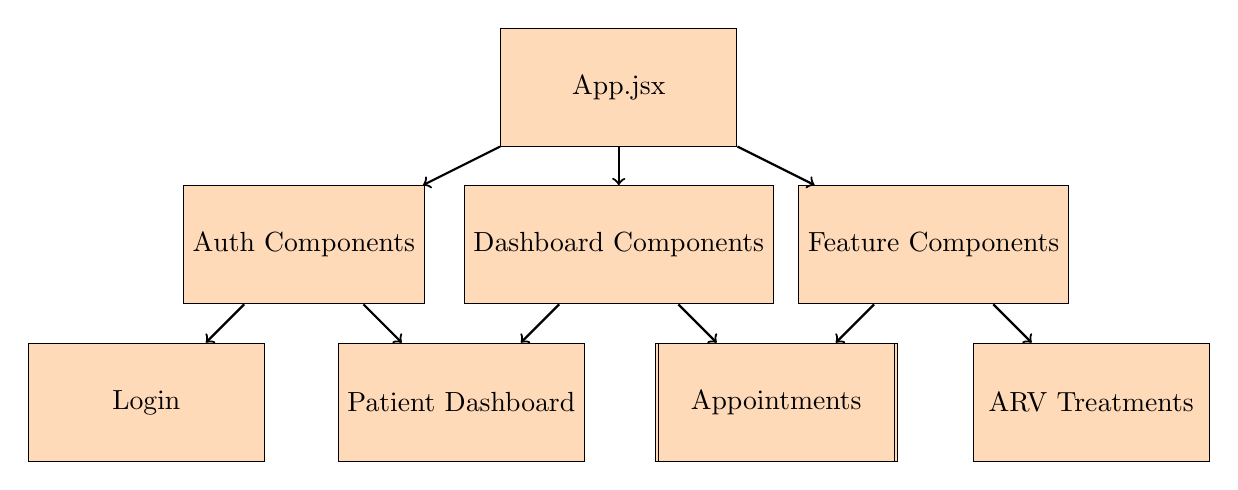
\begin{tikzpicture}[
    component/.style={draw, fill=classcolor, minimum width=3cm, minimum height=1.5cm, text centered},
    arrow/.style={->, thick}
]

% Main components
\node[component] (app) at (0, 0) {App.jsx};
\node[component] (auth) at (-4, -2) {Auth Components};
\node[component] (dashboard) at (0, -2) {Dashboard Components};
\node[component] (features) at (4, -2) {Feature Components};

% Sub-components
\node[component] (login) at (-6, -4) {Login};
\node[component] (register) at (-2, -4) {Register};

\node[component] (patient) at (-2, -4) {Patient Dashboard};
\node[component] (doctor) at (2, -4) {Doctor Dashboard};

\node[component] (appointments) at (2, -4) {Appointments};
\node[component] (treatments) at (6, -4) {ARV Treatments};

% Arrows
\draw[arrow] (app) -- (auth);
\draw[arrow] (app) -- (dashboard);
\draw[arrow] (app) -- (features);

\draw[arrow] (auth) -- (login);
\draw[arrow] (auth) -- (register);

\draw[arrow] (dashboard) -- (patient);
\draw[arrow] (dashboard) -- (doctor);

\draw[arrow] (features) -- (appointments);
\draw[arrow] (features) -- (treatments);

\end{tikzpicture}
\caption{Frontend Component Architecture}
\label{fig:frontend-architecture}
\end{figure}

\subsection{State Management}

The application uses React Context API for state management:

\begin{lstlisting}[language=JavaScript, caption=Authentication Context]
import React, { createContext, useContext, useReducer } from 'react';

const AuthContext = createContext();

const authReducer = (state, action) => {
  switch (action.type) {
    case 'LOGIN':
      return {
        ...state,
        user: action.payload.user,
        token: action.payload.token,
        isAuthenticated: true
      };
    case 'LOGOUT':
      return {
        ...state,
        user: null,
        token: null,
        isAuthenticated: false
      };
    default:
      return state;
  }
};

export const AuthProvider = ({ children }) => {
  const [state, dispatch] = useReducer(authReducer, {
    user: null,
    token: null,
    isAuthenticated: false
  });

  return (
    <AuthContext.Provider value={{ state, dispatch }}>
      {children}
    </AuthContext.Provider>
  );
};
\end{lstlisting}

\section{Security Design}

\subsection{Security Architecture}

The system implements multiple layers of security:

\begin{figure}[H]
\centering
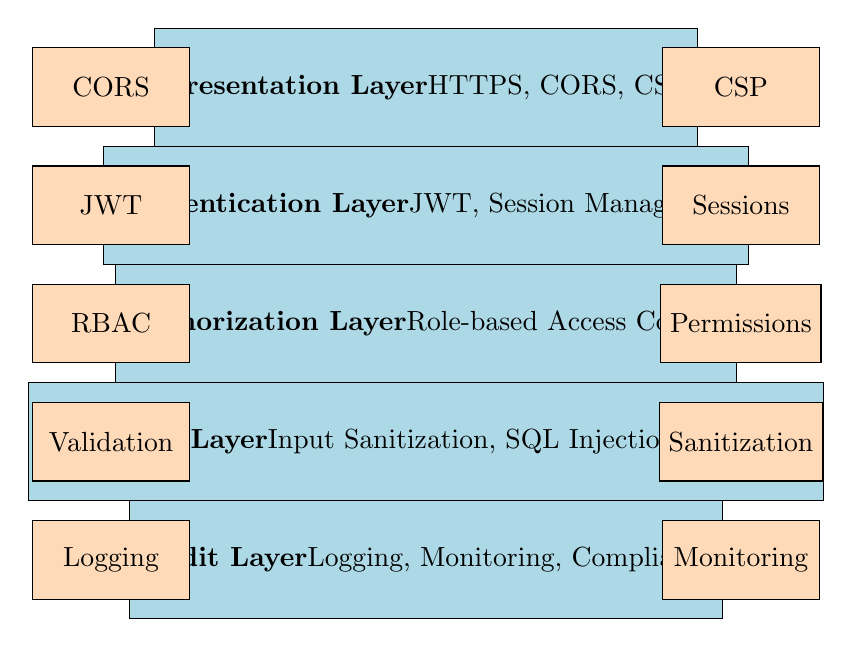
\begin{tikzpicture}[
    layer/.style={draw, fill=packagecolor, minimum width=6cm, minimum height=1.5cm, text centered},
    component/.style={draw, fill=classcolor, minimum width=2cm, minimum height=1cm, text centered},
    arrow/.style={->, thick}
]

% Security layers
\node[layer] (presentation) at (0, 4) {\textbf{Presentation Layer}\\HTTPS, CORS, CSP};
\node[layer] (authentication) at (0, 2.5) {\textbf{Authentication Layer}\\JWT, Session Management};
\node[layer] (authorization) at (0, 1) {\textbf{Authorization Layer}\\Role-based Access Control};
\node[layer] (validation) at (0, -0.5) {\textbf{Validation Layer}\\Input Sanitization, SQL Injection Prevention};
\node[layer] (audit) at (0, -2) {\textbf{Audit Layer}\\Logging, Monitoring, Compliance};

% Security components
\node[component] (cors) at (-4, 4) {CORS};
\node[component] (csp) at (4, 4) {CSP};

\node[component] (jwt) at (-4, 2.5) {JWT};
\node[component] (session) at (4, 2.5) {Sessions};

\node[component] (rbac) at (-4, 1) {RBAC};
\node[component] (permissions) at (4, 1) {Permissions};

\node[component] (validation) at (-4, -0.5) {Validation};
\node[component] (sanitization) at (4, -0.5) {Sanitization};

\node[component] (logging) at (-4, -2) {Logging};
\node[component] (monitoring) at (4, -2) {Monitoring};

\end{tikzpicture}
\caption{Security Architecture}
\label{fig:security-architecture}
\end{figure}

\subsection{Security Implementation}

\begin{lstlisting}[language=Java, caption=Security Configuration]
@Configuration
@EnableWebSecurity
@EnableMethodSecurity
public class SecurityConfig {
    
    @Bean
    public SecurityFilterChain filterChain(HttpSecurity http) throws Exception {
        http
            .csrf(csrf -> csrf.disable())
            .cors(cors -> cors.configurationSource(corsConfigurationSource()))
            .authorizeHttpRequests(auth -> auth
                .requestMatchers("/api/auth/**").permitAll()
                .requestMatchers("/api/admin/**").hasRole("ADMIN")
                .requestMatchers("/api/manager/**").hasRole("MANAGER")
                .requestMatchers("/api/doctor/**").hasRole("DOCTOR")
                .requestMatchers("/api/patient/**").hasRole("PATIENT")
                .anyRequest().authenticated()
            )
            .sessionManagement(session -> session
                .sessionCreationPolicy(SessionCreationPolicy.STATELESS)
            )
            .addFilterBefore(jwtRequestFilter, UsernamePasswordAuthenticationFilter.class);
        
        return http.build();
    }
}
\end{lstlisting}

\section{Performance and Scalability}

\subsection{Performance Optimization}

\begin{longtable}{|p{3cm}|p{3cm}|p{8cm}|}
\hline
\textbf{Component} & \textbf{Optimization} & \textbf{Description} \\
\hline
Database & Connection Pooling & HikariCP connection pool with optimized settings \\
\hline
Caching & Redis Integration & Session caching and frequently accessed data \\
\hline
API Response & Pagination & Large dataset pagination with configurable page sizes \\
\hline
Frontend & Code Splitting & React.lazy for component-level code splitting \\
\hline
Images & Compression & Image optimization and lazy loading \\
\hline
Queries & Indexing & Strategic database indexing for performance \\
\hline
\end{longtable}

\subsection{Scalability Considerations}

\begin{itemize}
    \item \textbf{Horizontal Scaling}: Stateless design allows horizontal scaling
    \item \textbf{Load Balancing}: Support for multiple application instances
    \item \textbf{Database Scaling}: Read replicas for read-heavy operations
    \item \textbf{Caching Strategy}: Multi-level caching for improved performance
    \item \textbf{Microservices Ready}: Modular design supports future microservices migration
\end{itemize}

\section{Testing Strategy}

\subsection{Testing Pyramid}

\begin{figure}[H]
\centering
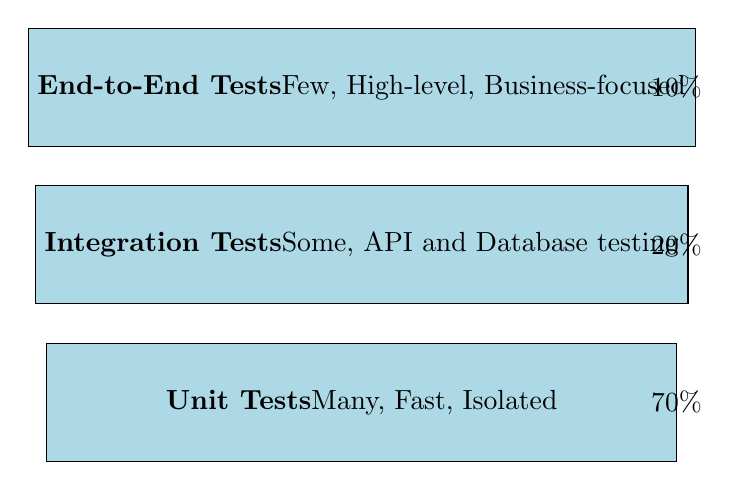
\begin{tikzpicture}[
    level/.style={draw, fill=packagecolor, minimum width=8cm, minimum height=1.5cm, text centered},
    arrow/.style={->, thick}
]

% Testing levels
\node[level] (e2e) at (0, 0) {\textbf{End-to-End Tests}\\Few, High-level, Business-focused};
\node[level] (integration) at (0, -2) {\textbf{Integration Tests}\\Some, API and Database testing};
\node[level] (unit) at (0, -4) {\textbf{Unit Tests}\\Many, Fast, Isolated};

% Coverage indicators
\node at (4, 0) {10\%};
\node at (4, -2) {20\%};
\node at (4, -4) {70\%};

\end{tikzpicture}
\caption{Testing Strategy Pyramid}
\label{fig:testing-pyramid}
\end{figure}

\subsection{Test Coverage Requirements}

\begin{longtable}{|p{3cm}|p{2cm}|p{9cm}|}
\hline
\textbf{Test Type} & \textbf{Coverage} & \textbf{Description} \\
\hline
Unit Tests & 85\%+ & Service layer, utility functions, and business logic \\
\hline
Integration Tests & 70\%+ & API endpoints, database operations, and external services \\
\hline
End-to-End Tests & 50\%+ & Critical user journeys and business workflows \\
\hline
Security Tests & 90\%+ & Authentication, authorization, and vulnerability testing \\
\hline
Performance Tests & 100\% & Load testing and performance benchmarking \\
\hline
\end{longtable}

\section{Deployment and DevOps}

\subsection{Deployment Architecture}

\begin{figure}[H]
\centering
\fbox{
\begin{minipage}{0.9\textwidth}
\centering
\vspace{3cm}
\textbf{HIV Clinic Management System - Deployment Diagram}\\
\vspace{0.5cm}
\textit{Comprehensive deployment diagram showing production environment setup, load balancers, application servers, database clusters, monitoring systems, and security components}\\
\vspace{0.5cm}
\textit{Dimensions: 24" x 16"}\\
\vspace{0.5cm}
\textit{Generated from: deployment\_diagram.plantuml}\\
\vspace{3cm}
\end{minipage}
}
\caption{System Deployment Diagram}
\label{fig:deployment-diagram}
\end{figure}

\subsection{CI/CD Pipeline}

\begin{lstlisting}[language=YAML, caption=GitHub Actions Workflow]
name: CI/CD Pipeline

on:
  push:
    branches: [ main, develop ]
  pull_request:
    branches: [ main ]

jobs:
  test:
    runs-on: ubuntu-latest
    steps:
    - uses: actions/checkout@v3
    - name: Set up JDK 17
      uses: actions/setup-java@v3
      with:
        java-version: '17'
    - name: Run Backend Tests
      run: mvn test
    - name: Run Frontend Tests
      run: npm test
    - name: Build Application
      run: mvn clean package

  deploy:
    needs: test
    runs-on: ubuntu-latest
    if: github.ref == 'refs/heads/main'
    steps:
    - name: Deploy to Production
      run: |
        # Deployment steps
        echo "Deploying to production..."
\end{lstlisting}

\section{Monitoring and Maintenance}

\subsection{Health Monitoring}

The system implements comprehensive health monitoring:

\begin{lstlisting}[language=Java, caption=Health Check Endpoint]
@RestController
@RequestMapping("/api/health")
public class HealthController {
    
    @GetMapping
    public ResponseEntity<Map<String, Object>> healthCheck() {
        Map<String, Object> health = new HashMap<>();
        health.put("status", "UP");
        health.put("timestamp", LocalDateTime.now());
        health.put("version", "1.0.0");
        health.put("database", checkDatabaseHealth());
        health.put("services", checkServiceHealth());
        
        return ResponseEntity.ok(health);
    }
    
    private String checkDatabaseHealth() {
        // Database connectivity check
        return "UP";
    }
    
    private Map<String, String> checkServiceHealth() {
        // Service health checks
        return Map.of(
            "authentication", "UP",
            "appointments", "UP",
            "notifications", "UP"
        );
    }
}
\end{lstlisting}

\subsection{Logging Strategy}

\begin{longtable}{|p{3cm}|p{2cm}|p{9cm}|}
\hline
\textbf{Log Level} & \textbf{Usage} & \textbf{Description} \\
\hline
ERROR & Critical failures & System errors, exceptions, and critical failures \\
\hline
WARN & Potential issues & Warning conditions and potential problems \\
\hline
INFO & General information & Important business events and system state changes \\
\hline
DEBUG & Development & Detailed debugging information for development \\
\hline
TRACE & Detailed debugging & Very detailed debugging information \\
\hline
\end{longtable}

\section{Conclusion}

The HIV Clinic Management System is designed with modern software engineering principles, ensuring scalability, security, and maintainability. The system architecture supports the complex requirements of healthcare management while maintaining high performance and reliability standards.

Key design decisions include:

\begin{itemize}
    \item \textbf{Layered Architecture}: Clear separation of concerns with Spring Boot backend and React frontend
    \item \textbf{Security First}: Comprehensive security implementation with JWT authentication and role-based access control
    \item \textbf{Scalable Design}: Stateless architecture supporting horizontal scaling
    \item \textbf{Comprehensive Testing}: Multi-level testing strategy ensuring code quality
    \item \textbf{Modern Technologies}: Java 17, Spring Boot 3.2, React 18, and SQL Server
    \item \textbf{Healthcare Compliance}: Design considerations for medical data privacy and security
\end{itemize}

The system is ready for production deployment with proper monitoring, logging, and maintenance procedures in place.

\end{document}